\section{Testing AI Systems}
As in the classic software design process, testing is a crucial step in building AI systems, 
but it also has unique challenges and considerations due to the nature of LLMs and their non-deterministic outputs.
\\
The usual testing process involves the following steps:
\begin{itemize}
    \item \textbf{Define Test Cases}: Identify a set of inputs and expected outputs that cover a range of scenarios, including edge cases and common use cases.
    \item \textbf{Analyze Outputs}: check the failing tests and iterate on the source code or prompt to fix them.
\end{itemize}
However, when testing AI systems, we need to consider additional factors:
\begin{itemize}
    \item \textbf{Problem Complexity}: usually AI systems are designed to handle complex problems, where no
    single correct answer exists, and the value comes from handling ambiguity and generating creative solutions.
    In such cases, defining expected outputs can be challenging;
    \item \textbf{Overfitting to Test Cases}: If you design your prompt to pass specific test cases, 
    you might end up with a prompt that performs well on those cases but fails to generalize to new inputs.
\end{itemize}
We can think of different approaches to tackle these challenges and improve the testing results of the system. 
In the following sections, we will explore some of these approaches.

\subsection{Single Shot Prompts}
The first idea is to use single shot prompts, where the failing test cases are directly included in the prompt as examples of what not to do, or as examples of the desired output format.
This can help the model understand the specific requirements and constraints of the task, and improve its performance.
\\\\
However, this approach can also lead to overfitting if the prompt becomes too tailored to the specific test cases, and it may not generalize well to new inputs, leading
to terrible performance when put in production.
\\
A general rule of thumb is to \textbf{NEVER include test cases in the prompt} and to never design the prompt to pass specific test cases. 
The best strategy would be to design the prompt without even knowing what the test cases are.

\subsection{Self-Critique}
Another approach is to use self-critique, where, in the same prompt, the model is asked to evaluate its own output and identify any errors or inconsistencies.
This can help improve the reliability of the output, as the model can catch and correct its own mistakes.
\\\\
A better approach is to use a separate prompt for self-critique (if possible, also with a different model), where the model is given the original output and
asked to evaluate it and to provide a revised version of the output if necessary.
Using a separate prompt allows the model to focus solely on the critique process, removing all the previous context and potential biases from the original prompt.

\subsection{Feedback Loops}
A more advanced approach is to use feedback loops. 
You can design a system where the model generates an output, then evaluates it 
against the test cases, and iteratively refines the system prompt to improve performance.
There are different strategies to implement feedback loops.

\begin{figure}[htbp]
    \centering
    \IfFileExists{../../Tikz/feedback-loop.tex}{
        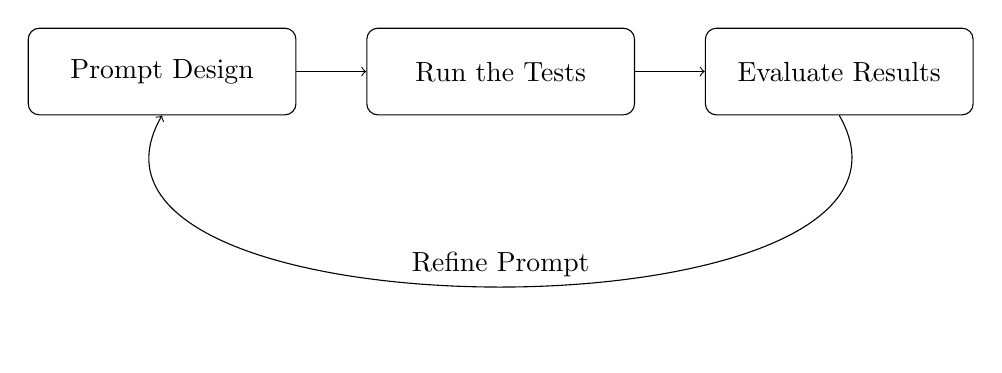
\begin{tikzpicture}
    \node[draw, rectangle, rounded corners, minimum width=3.4cm, minimum height=1.1cm] (prompt) at (0,0) {Prompt Design};
    \node[draw, rectangle, rounded corners, minimum width=3.4cm, minimum height=1.1cm] (execute) at (4.3,0) {Run the Tests};
    \node[draw, rectangle, rounded corners, minimum width=3.4cm, minimum height=1.1cm] (evaluate) at (8.6,0) {Evaluate Results};

    \draw[->] (prompt) -- (execute);
    \draw[->] (execute) -- (evaluate);
    \draw[->] (evaluate.south) to[out=-60, in=-120] node[above] {Refine Prompt} (prompt.south);
\end{tikzpicture}
    }{
        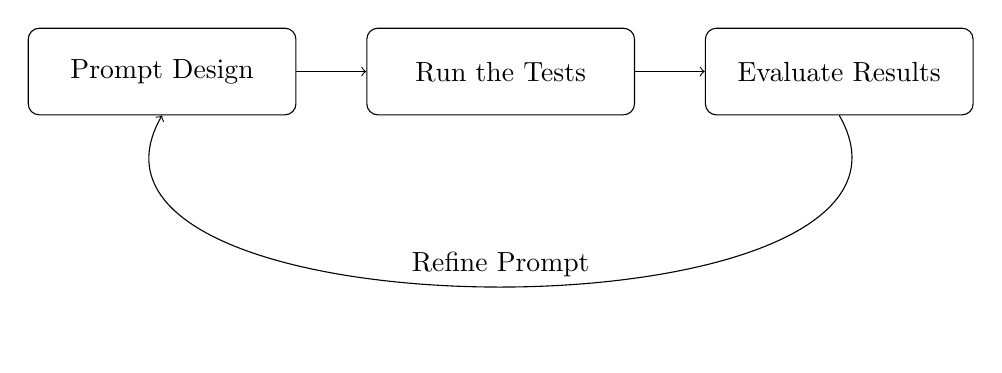
\begin{tikzpicture}
    \node[draw, rectangle, rounded corners, minimum width=3.4cm, minimum height=1.1cm] (prompt) at (0,0) {Prompt Design};
    \node[draw, rectangle, rounded corners, minimum width=3.4cm, minimum height=1.1cm] (execute) at (4.3,0) {Run the Tests};
    \node[draw, rectangle, rounded corners, minimum width=3.4cm, minimum height=1.1cm] (evaluate) at (8.6,0) {Evaluate Results};

    \draw[->] (prompt) -- (execute);
    \draw[->] (execute) -- (evaluate);
    \draw[->] (evaluate.south) to[out=-60, in=-120] node[above] {Refine Prompt} (prompt.south);
\end{tikzpicture}
    }
    \caption{Feedback loop for prompt testing and refinement.}
    \label{fig:testing-feedback-loop}
\end{figure}

\subsubsection{Human in the loop}
In the basic implementation of feedback loops, a human is involved in three steps of the process:
\begin{itemize}
    \item \textbf{Prompt Design}: The human designs the initial prompt based on their understanding of the task and the requirements;
    \item \textbf{Evaluate Results}: After executing the prompt on a set of test cases, the human evaluates the results and identifies 
    any errors or inconsistencies;
    \item \textbf{Refine Prompt}: Based on the evaluation, the human refines the prompt to improve its performance.
\end{itemize}
We can see how this process can be time-consuming and inefficient, especially if the prompt requires multiple iterations to achieve the desired performance.
Not only from a time perspective, but also from the knowledge perspective: the human needs to understand the model's behavior and how to design effective prompts,
which can be a complex task in itself.
\\\\
Replacing human evaluation with an LLM judge is the key step to make the loop scalable.

\subsubsection{Automatic Feedback Loops}
In a fully automated feedback loop, the model itself is responsible for evaluating its own output and refining the prompt accordingly.
They are based on the idea of using \textbf{LLMs as judges}, where the human is replaced by the model, 
which is given a set of test cases and asked to evaluate its own output against those cases.
It is then asked to provide feedback on how to improve the prompt, and to generate a revised version of the prompt itself, leading to the automatic loop process.

\paragraph{LLM as a Judge}
Defining a good prompt for the LLM judge is not trivial, and it is crucial to ensure an improved performance of the system.
Usually we are interested in defining a score for each parameter we want to evaluate.
Based on this, we can also filter out the outputs that do not meet a certain threshold, and manually review them to understand the weaknesses of the system.
\\\\
Since its cruciality, the model used for this task should be the best available, and it should be different 
from the one used for the original prompt, to avoid bias and to ensure a more objective evaluation.

\paragraph{Prompt Improvement}
The prompt improvement step is also crucial, as it is the one that allows the system to learn and improve over time.
One of the common approaches is to ask the model to provide many variations of the original prompt (following known prompting strategies),
and then to evaluate those variations against the test cases, selecting the best performing one as the new prompt for the next iteration.
\\
Supposing that the Judge is correctly evaluating the outputs, this process can lead to a significant improvement in performance over time.

\paragraph{Wrong approach - Vibe Eval}
A common mistake is to not implement the Judge, but to have a person testing a few cases manually to check the
quality of the system, and to rely on their "vibe" to decide whether the system is good or not.
This approach is obviously not scalable, and it also tends to produce prompts that overfit to the specific test cases.

\paragraph{Avoid Overfitting}
The automatic approach can still lead to overfitting with small enough test sets, or after a certain number of iterations.
It's important, after each iteration, to increase the size of the test set, to ensure that the system is not just learning to 
pass a small set of cases, but is actually improving its generalization capabilities.

\paragraph{Technical Suggestions}
In practice, when implementing feedback loops, it is important to consider the following technical suggestions:
\begin{itemize}
    \item \textbf{Use a separate model for the Judge}: This helps to avoid bias and ensures a more objective evaluation of the outputs.
    The best available model should be used for this task, as the quality of the evaluation is crucial for the improvement of the system.
    \item \textbf{Define clear evaluation criteria}: The prompt for the Judge should include clear criteria for evaluating the outputs. 
    Also, it should be designed as the first step of the process;
    \item \textbf{Batch testing}: Usually testing is done in batches, where a set of test cases is evaluated at once.
    There are different strategies to implement batch testing:
    \begin{itemize}
        \item \textbf{Trust the Judge}: You can simply ask the Judge to provide a list of elements as output, 
        and then match it with the expected outputs assuming they keep the same order. 
        This is the simplest approach, but even stronger models can make mistakes in this type of tasks, leading to incorrect evaluations.
        \item \textbf{Use IDs}: A more robust approach is to assign an ID to each test case, and ask the Judge to repeat the ID in the output. 
        This way, we can always map the output back to the original test cases. It's important to also use short IDs, so that the models
        sees them as a single token.
    \end{itemize}
\end{itemize}